“转糖盘”是一个固定不动的圆盘,盘面被平分为$10$格(如图),在偶数格内放一块糖,在奇数格内放上值钱的物品.某人给摊主$5$角钱,即可沿着顺时针方向转动圆盘一次.圆盘停转后指针指到哪一格,摊主便依据该格的数顺着转盘转动方向从下一格起数格,数到哪一格,该格中的物品就归这个人.例如,指针停在$3$,则从$4$起再数$3$格,即第$6$格中的物品就是奖品.实际上,不管你怎么转,永远拿不到奇数格中的物品.请你试着填写下面表格.看看你的奖品是什么?\\
\begin{center}
	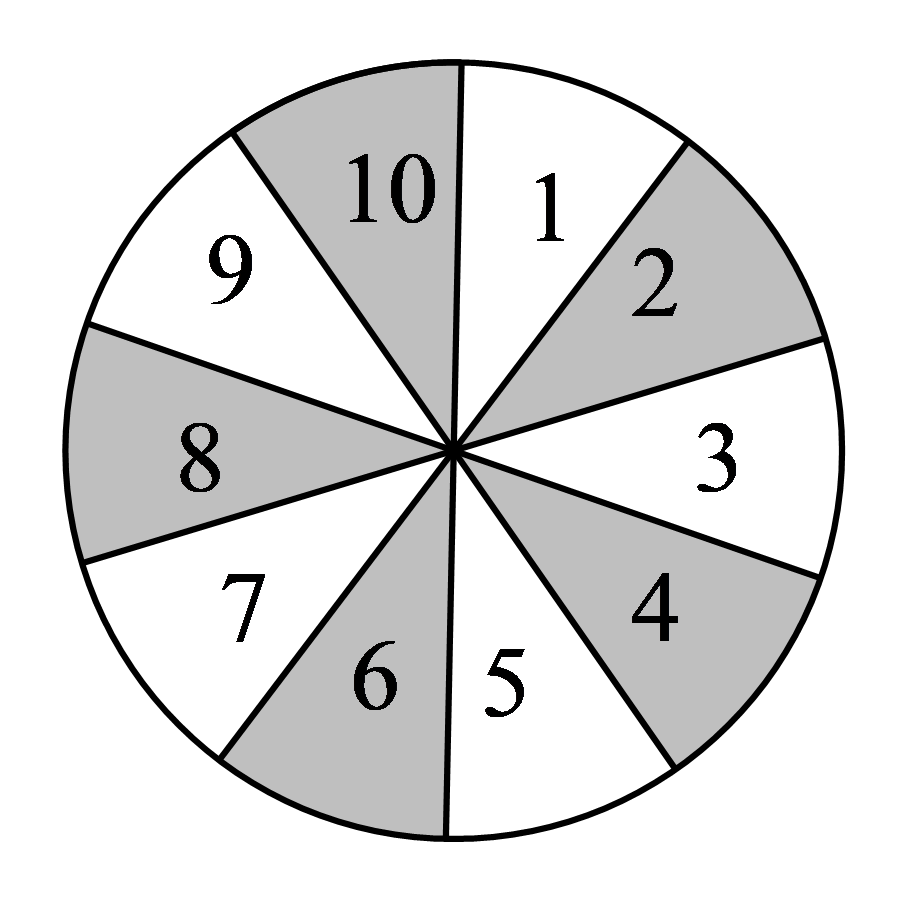
\includegraphics[width=4cm]{lib/image/MJA01030110.png}
	\captionof{figure}{第10题图}
	\vspace{0.5cm}
\end{center}

\begin{tabular}{|l|l|l|l|l|l|l|l|l|l|l|}
	\hline
	指针所在格数 &     &     &     &     &     &     &     &     &     &  \\ \hline
	奖品所在格数 &     &     &     &     &     &     &     &     &     &  \\ \hline
\end{tabular}